% \documentclass[aspectratio=169,notes]{beamer}
\documentclass[aspectratio=169]{beamer}
\usetheme[faculty=phil]{fibeamer}
\usepackage{polyglossia}
\setmainlanguage{english} %% main locale instead of `english`, you
%% can typeset the presentation in either Czech or Slovak,
%% respectively.
\setotherlanguages{russian} %% The additional keys allow
%%
%%   \begin{otherlanguage}{czech}   ... \end{otherlanguage}
%%   \begin{otherlanguage}{slovak}  ... \end{otherlanguage}
%%
%% These macros specify information about the presentation
\title[Introduction to Robotics (In2Ro)]{Introduction to Robotics, Lecture 6} %% that will be typeset on the
\subtitle{Programming real manipulators 
\\ Path planning \\ Trajectory planning  } %% title page.
\author{Oleg Bulichev}
%% These additional packages are used within the document:
\usepackage{ragged2e}  % `\justifying` text
\usepackage{booktabs}  % Tables
\usepackage{tabularx}
\usepackage{tikz}      % Diagrams
\usetikzlibrary{calc, shapes, backgrounds, trees, positioning, arrows.meta}
\usetikzlibrary{decorations.pathreplacing,calligraphy,calc,graphs}
\usepackage{amsmath, amssymb}
\usepackage{url}       % `\url`s
\usepackage{listings}  % Code listings
\usepackage{floatrow}
\usepackage{subcaption}
\usepackage{mathtools}
\usepackage{todonotes}
\usepackage{fontspec}
\usepackage{multicol}
\usepackage{pdfpages}
\usepackage{wrapfig}
\usepackage{qrcode}
\usepackage{animate}
\usepackage{booktabs}
\usepackage{multirow}
\usepackage{graphicx}
\usepackage{colortbl}

\graphicspath{{resources/}}
\frenchspacing

\setbeamertemplate{caption}{\raggedright\insertcaption\par}
\usetikzlibrary{graphs}

% \usepackage[backend=biber,style=ieee,autocite=footnote]{biblatex}
% \addbibresource{biblio.bib}
% \DefineBibliographyStrings{english}{%
%   bibliography = {References},}

\newcommand{\oleg}[2][] {\todo[color=red, #1] {OLEG:\\ #2}}
\newcommand{\fbckg}[1]{\usebackgroundtemplate{\includegraphics[width=\paperwidth]{#1}}}%frame background

\usepackage[framemethod=TikZ]{mdframed}
\newcommand{\dbox}[1]{
\begin{mdframed}[roundcorner=3pt, backgroundcolor=yellow, linewidth=0]
\vspace{1mm}
{#1}
\vspace{1mm}
\end{mdframed}
}

\begin{document}
\setlength{\abovedisplayskip}{0pt}
\setlength{\belowdisplayskip}{0pt}
\setlength{\abovedisplayshortskip}{0pt}
\setlength{\belowdisplayshortskip}{0pt}

\fbckg{fibeamer/figs/title_page.png}
\frame[c]{\setcounter{framenumber}{0}
    \usebeamerfont{title}%
    \usebeamercolor[fg]{title}%
    \begin{minipage}[b][6.5\baselineskip][b]{\textwidth}%
        \textcolor{black}{\raggedright\inserttitle}
    \end{minipage}
    % \vskip-1.5\baselineskip

    \usebeamerfont{subtitle}%
    \usebeamercolor[fg]{framesubtitle}%
    \begin{minipage}[b][3\baselineskip][b]{\textwidth}
        \raggedright%
        \insertsubtitle%
    \end{minipage}
    \vskip.25\baselineskip
}

\fbckg{fibeamer/figs/common.png}

\begin{frame}[t]{Why are two target poses not enough?}
    \begin{columns}[T,onlytextwidth]
        \begin{column}{0.49\textwidth}
            \begin{block}{The same start and goal}
                Which path should the robot follow?\\
                How fast should it move?\\
                What happens between the targets?
            \end{block}
            A target does not specify the complete motion.
        \end{column}
        \begin{column}{0.49\textwidth}
            \centering
            \begin{tikzpicture}[scale=1.05,>=Latex]
                \fill (0,0) circle (2pt) node[left] {$A$};
                \fill (3.3,2) circle (2pt) node[right] {$B$};
                \draw[blue,thick,->] (0,0)--(3.3,2);
                \draw[orange,thick,->] (0,0) to[out=90,in=180] (3.3,2);
                \draw[teal,thick,->] (0,0)--(2.7,0)--(3.3,2);
            \end{tikzpicture}
            \begin{block}{From a task to motion}
                Task $\to$ path $\to$ timing law $\to$ execution
            \end{block}
        \end{column}
    \end{columns}
\end{frame}

\begin{frame}[t]{Teach, store, repeat}
    \begin{columns}[T,onlytextwidth]
        \begin{column}{0.49\textwidth}
            \begin{block}{Teaching a motion}
                Guide the robot or move it with a teach pendant. Store positions or a recorded motion.
            \end{block}
            \begin{block}{Playback}
                Repeat the stored sequence; interpolate between taught positions.
            \end{block}
        \end{column}
        \begin{column}{0.49\textwidth}
            \[q_0\ \longrightarrow\ q_1\ \longrightarrow\ \cdots\ \longrightarrow\ q_n\]
            \begin{itemize}
                \item The program assumes that the scene stays as taught.
                \item A moved workpiece does not automatically change the program.
                \item Task feedback requires additional sensing and logic.
            \end{itemize}
            \small Internal motion feedback and adaptation to the scene are different levels.
        \end{column}
    \end{columns}
\end{frame}

\begin{frame}[t]{From taught points to a robot program}
    \begin{columns}[T,onlytextwidth]
        \begin{column}{0.49\textwidth}
            \begin{block}{A sequence of actions}
                Move to a pose.\\
                Perform an operation.\\
                Read an input.\\
                Choose the next action.
            \end{block}
            Conditions and loops make a program more than a list of points.
        \end{column}
        \begin{column}{0.49\textwidth}
            \begin{block}{Industrial robot languages}
                KUKA: KRL\\
                Universal Robots: URScript
            \end{block}
            A program combines motion commands with interaction with other equipment.
            \medskip

            Motion primitives still leave interpolation and execution to the controller.
        \end{column}
    \end{columns}
\end{frame}

\begin{frame}[t]{The pendant and an external computer}
    \small
    \begin{columns}[T,onlytextwidth]
        \begin{column}{0.49\textwidth}
            \begin{block}{Program and execute}
                \textbf{PolyScope}: build and run a program on the pendant.\\
                \textbf{URScript}: express motion and program logic for the robot controller.
            \end{block}
            \begin{block}{Exchange and integrate}
                \textbf{RTDE}: exchange robot state and configured input/output data.\\
                \textbf{ROS driver}: connect the robot to external robotics software.
            \end{block}
        \end{column}
        \begin{column}{0.49\textwidth}
            \begin{block}{Why connect a computer?}
                Log measurements, calculate a plan, use sensors, or implement task feedback.
            \end{block}
            External computation $\leftrightarrow$ communication interface $\leftrightarrow$ controller program
            \medskip

            \alert{A communication interface is not a control law.}
            \medskip

            \href{https://www.universal-robots.com/articles/ur/interface-communication/overview-of-client-interfaces/}{\textcolor{blue}{UR: overview of client interfaces}}
        \end{column}
    \end{columns}
\end{frame}

\begin{frame}[c]
    \centering
    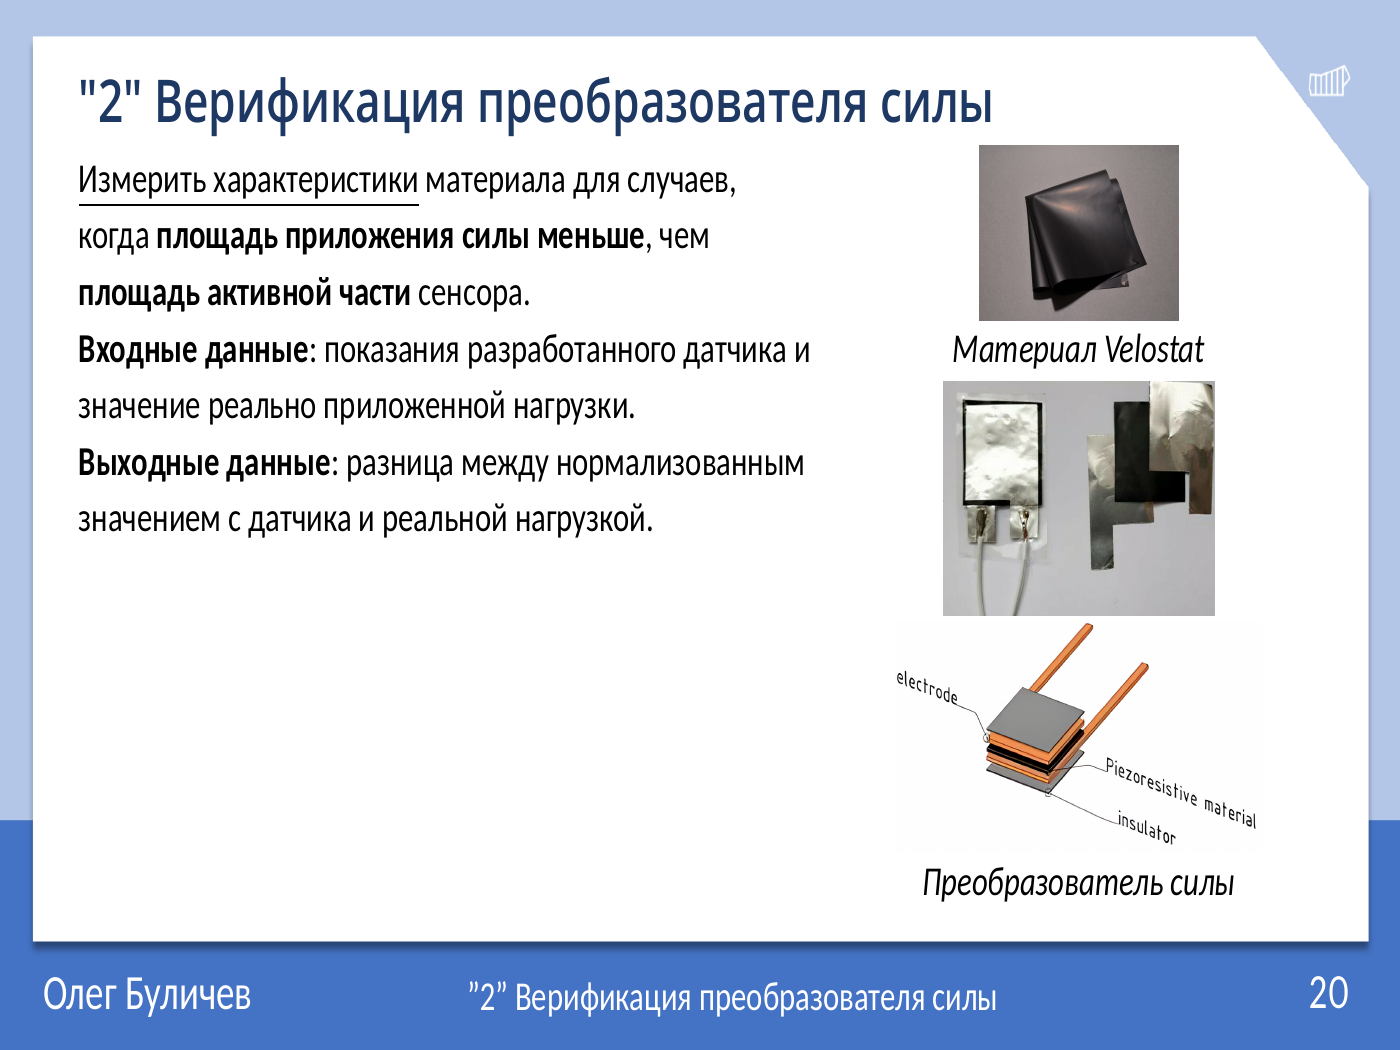
\includegraphics[width=\textwidth,height=0.8\paperheight,keepaspectratio]{ob_defence_p021.png}
\end{frame}

\begin{frame}[c]
    \centering
    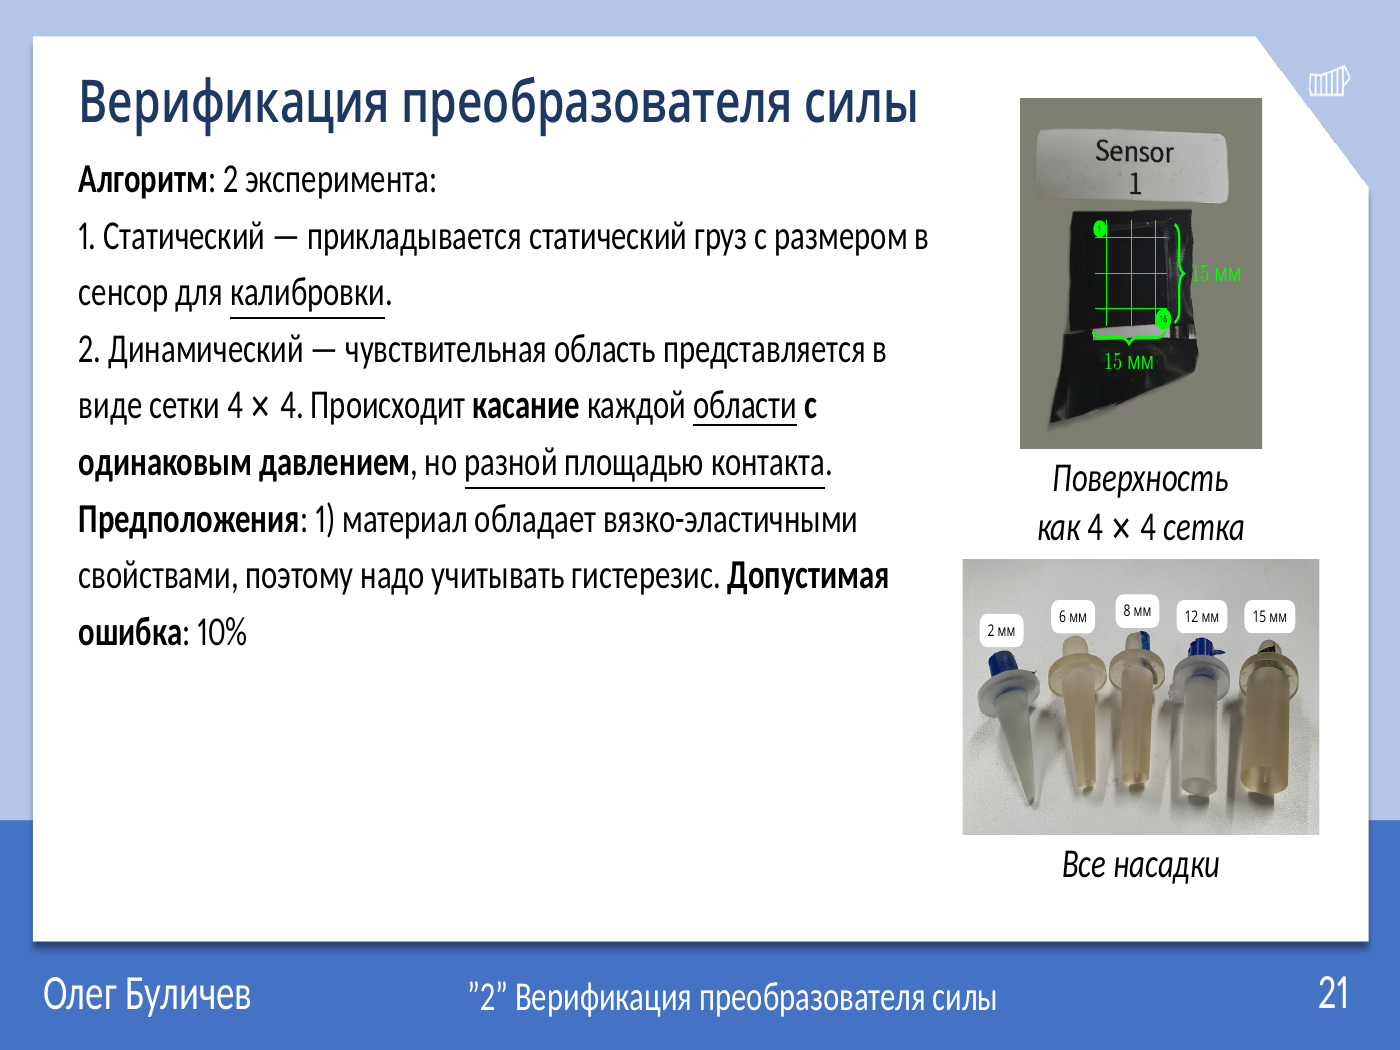
\includegraphics[width=\textwidth,height=0.8\paperheight,keepaspectratio]{ob_defence_p022.png}
\end{frame}

\begin{frame}[c]
    \centering
    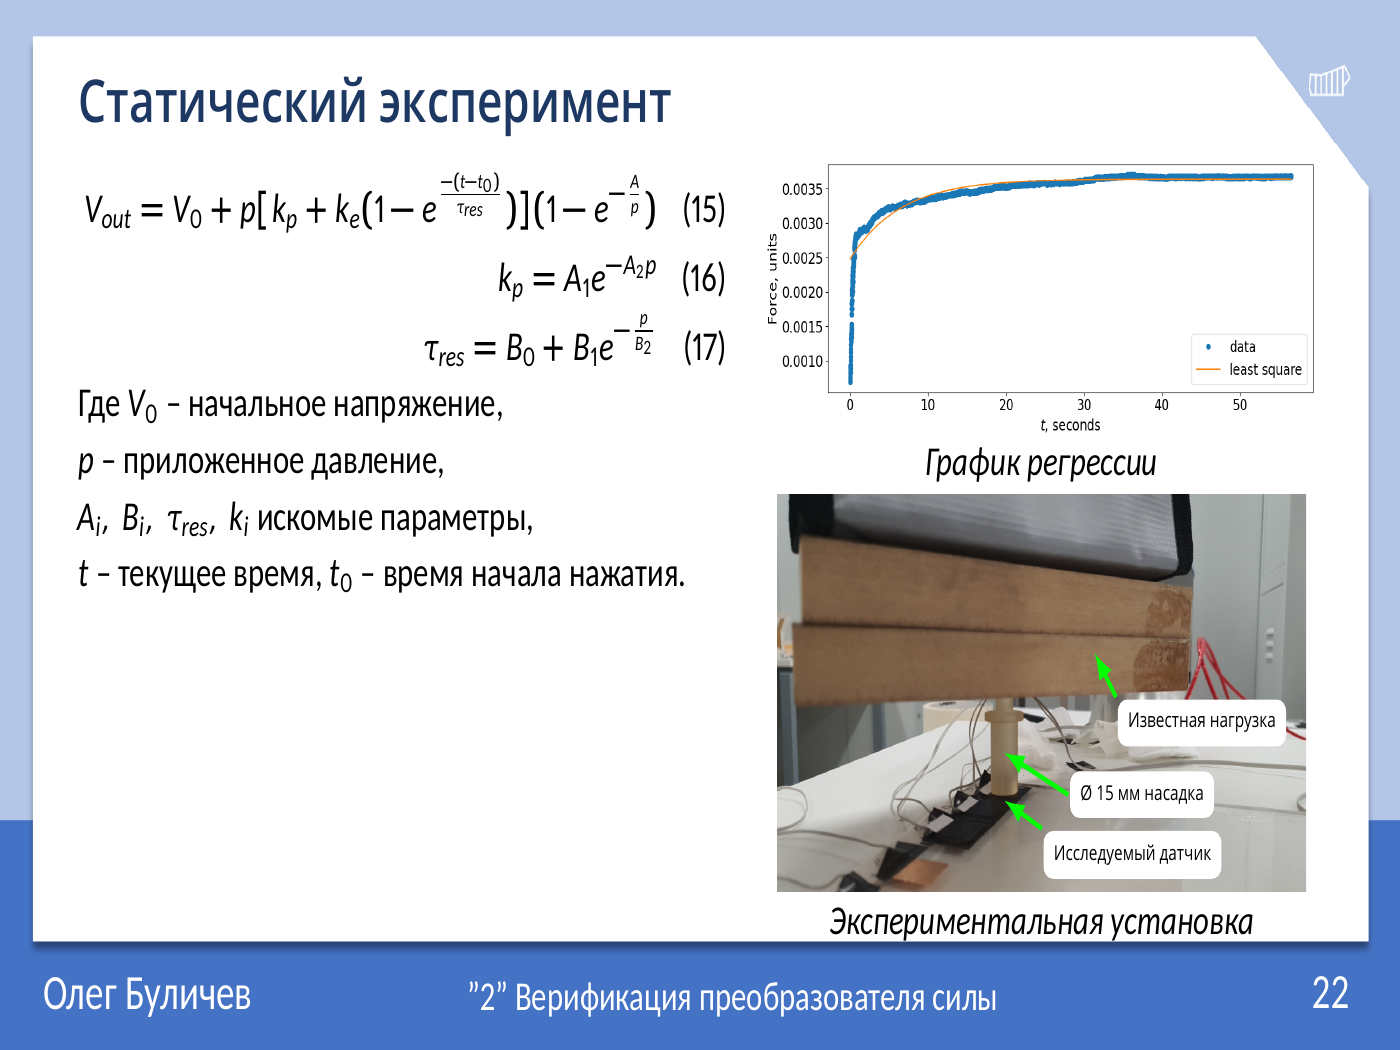
\includegraphics[width=\textwidth,height=0.8\paperheight,keepaspectratio]{ob_defence_p023.png}
\end{frame}

\begin{frame}[c]
    \centering
    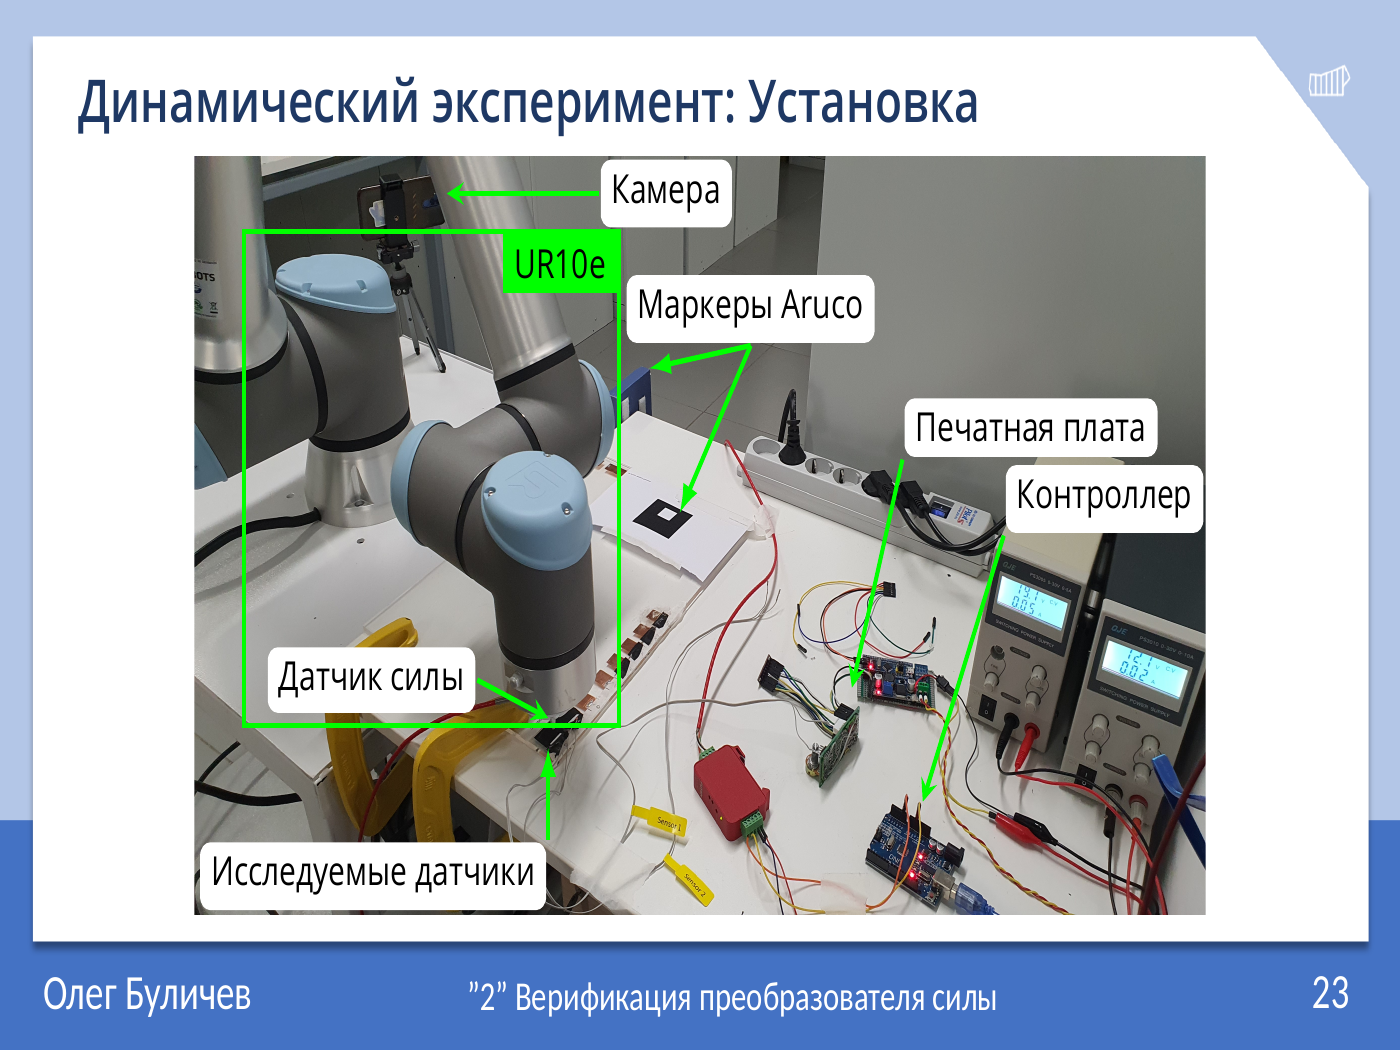
\includegraphics[width=\textwidth,height=0.8\paperheight,keepaspectratio]{ob_defence_p024.png}
\end{frame}

\begin{frame}[c]
    \centering
    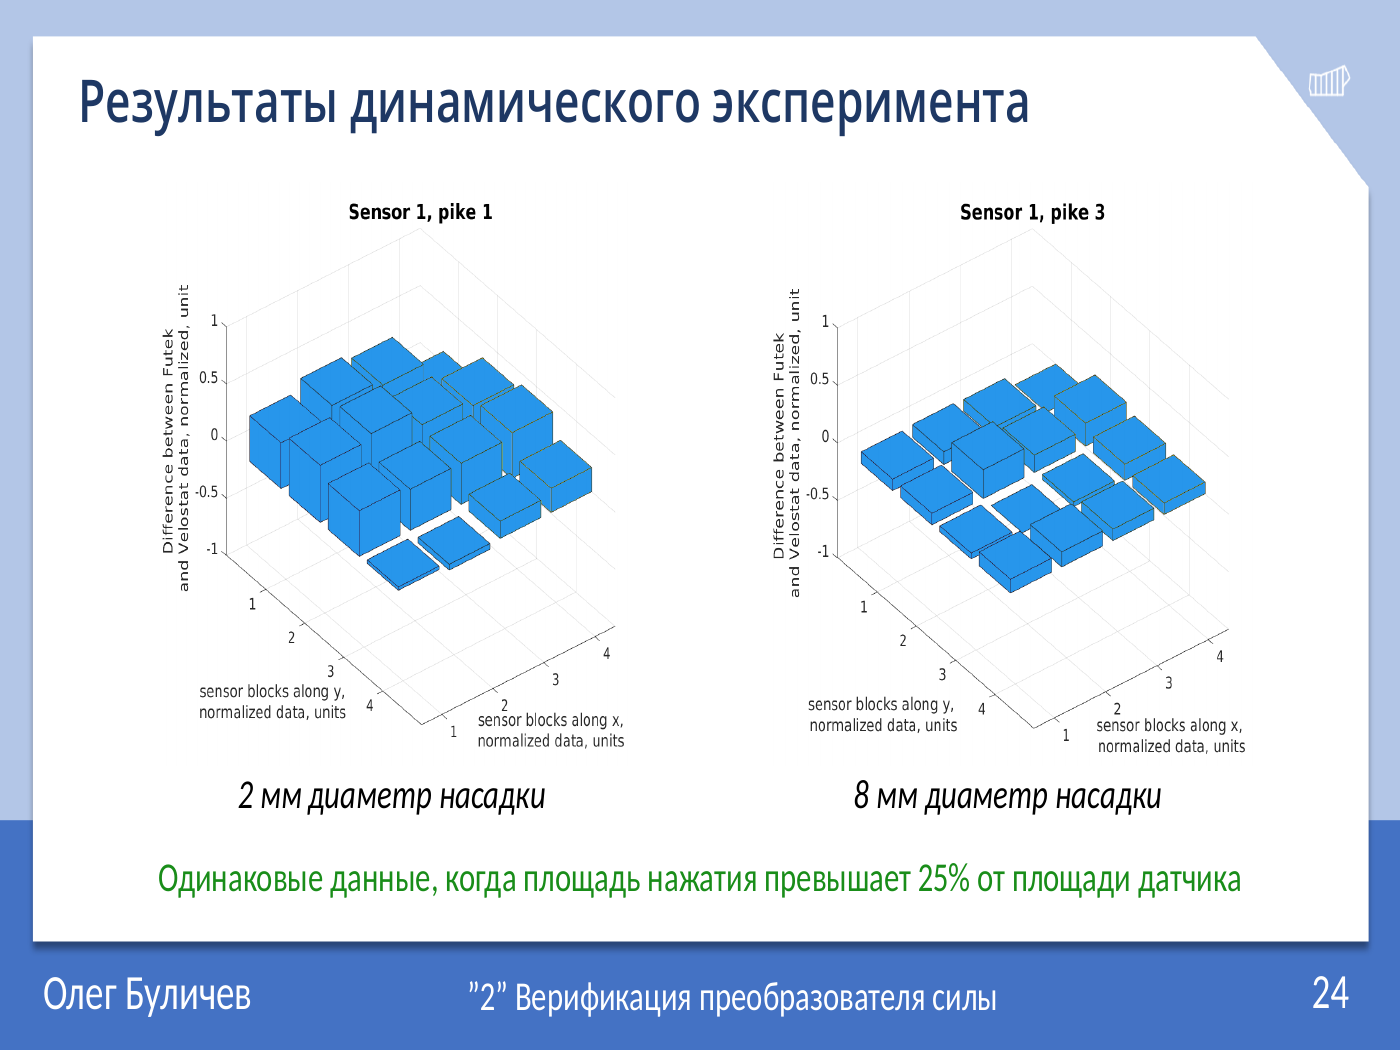
\includegraphics[width=\textwidth,height=0.8\paperheight,keepaspectratio]{ob_defence_p025.png}
\end{frame}

\begin{frame}[c]
    \centering
    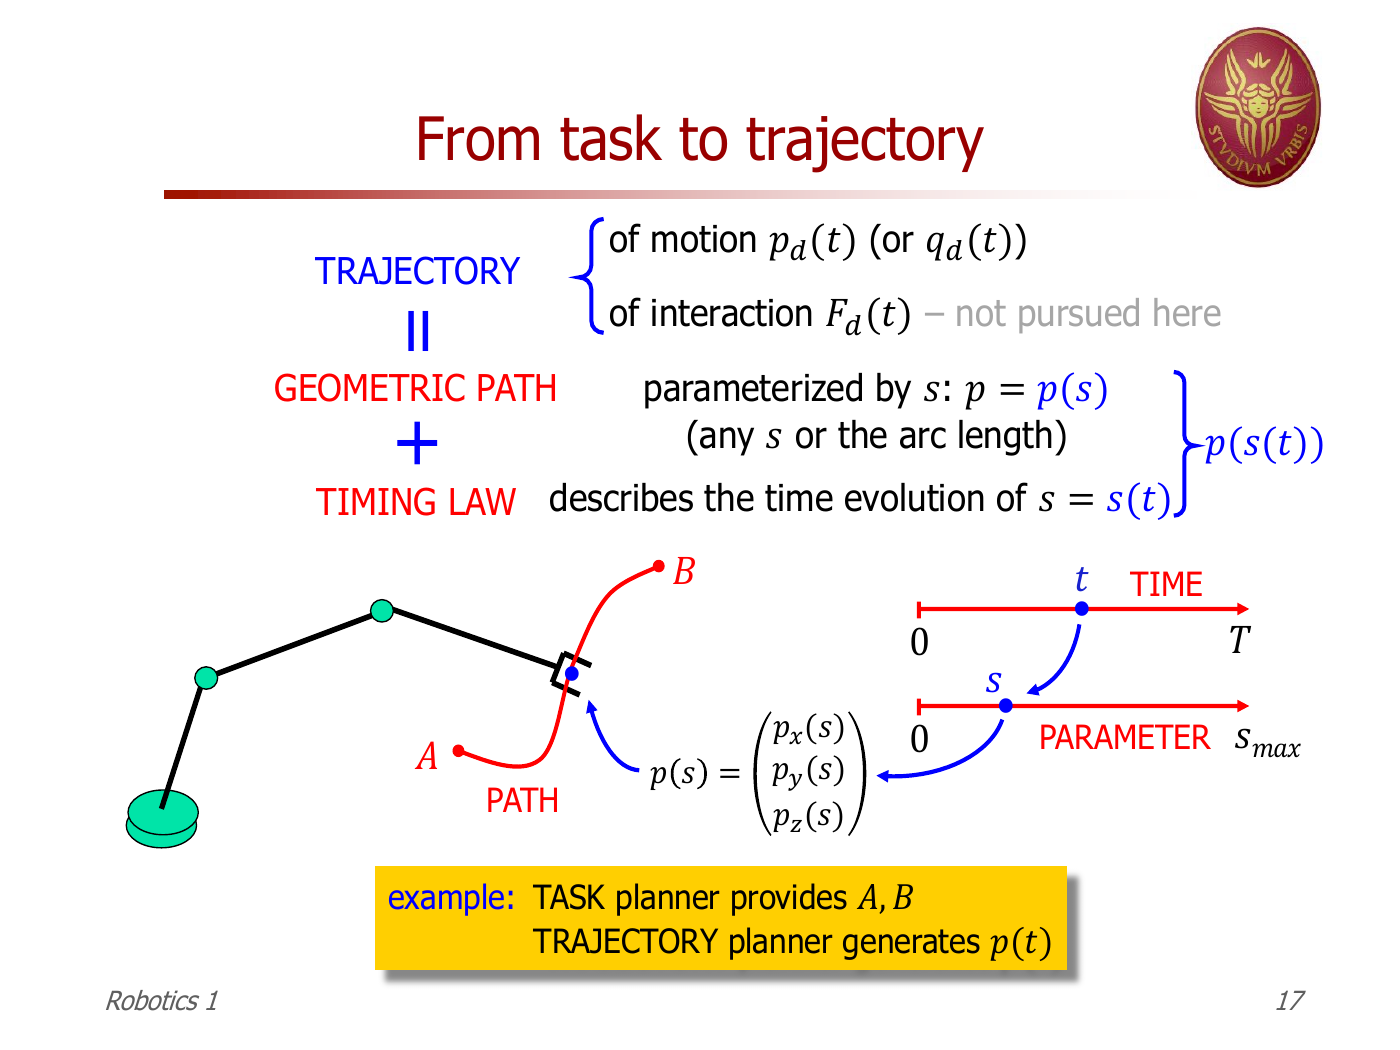
\includegraphics[width=\textwidth,height=0.8\paperheight,keepaspectratio]{dl13_p017_source.png}
\end{frame}

\begin{frame}[t]{Two spaces for planning the same transfer}
    \small
    \begin{columns}[T,onlytextwidth]
        \begin{column}{0.49\textwidth}
            \textbf{Joint space}
            \[q(s)=q_0+s(q_f-q_0)\]
            \centering
            \begin{tikzpicture}[scale=1.1]
                \draw[blue,very thick] (0,0)--(1,0)--(1,1);
                \draw[orange,very thick] (0,0)--(0,1)--(-0.707,1.707);
                \draw[teal,thick,domain=0:1,samples=50] plot ({cos(90*\x)+cos(90+45*\x)},{sin(90*\x)+sin(90+45*\x)});
                \fill (0,0) circle (2pt);
                \node[right] at (1,1) {$A$};
                \node[left] at (-0.707,1.707) {$B$};
            \end{tikzpicture}
            \par\raggedright A joint-space line usually produces a curved TCP path. Compute it with FK.
        \end{column}
        \begin{column}{0.49\textwidth}
            \textbf{Cartesian space}
            \[p(s)=p_0+s(p_f-p_0)\]
            \centering
            \begin{tikzpicture}[scale=1.1]
                \draw[blue,very thick] (0,0)--(1,0)--(1,1);
                \draw[orange,very thick] (0,0)--(0,1)--(-0.707,1.707);
                \draw[teal,thick] (1,1)--(-0.707,1.707);
                \fill (0,0) circle (2pt);
                \node[right] at (1,1) {$A$};
                \node[left] at (-0.707,1.707) {$B$};
            \end{tikzpicture}
            \par\raggedright A TCP line needs IK along the path and a continuous solution branch.
        \end{column}
    \end{columns}
\end{frame}

\begin{frame}[c]
    \centering
    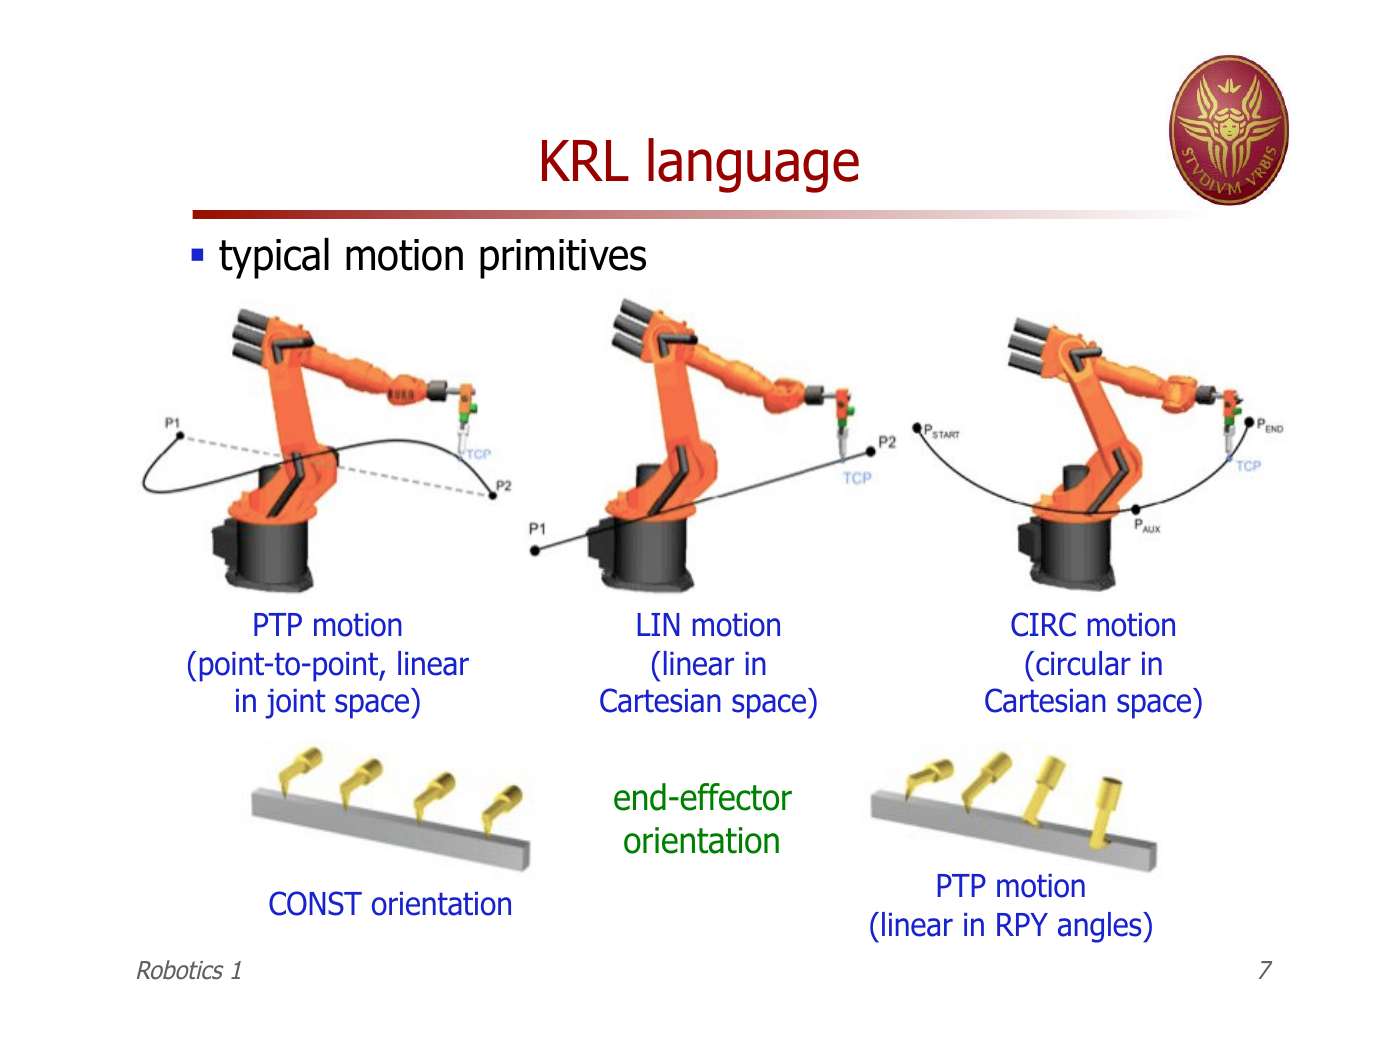
\includegraphics[width=\textwidth,height=0.75\paperheight,keepaspectratio]{dl06_p007_source.png}
    \par\small KUKA example. UR equivalents are introduced on the next slide.
\end{frame}

\begin{frame}[t]{Motion primitives on Universal Robots}
    \small
    \begin{columns}[T,onlytextwidth]
        \begin{column}{0.49\textwidth}
            \begin{block}{From the KUKA example to UR}
                PTP $\longrightarrow$ \textbf{MoveJ}: joint-space motion.\\
                LIN $\longrightarrow$ \textbf{MoveL}: linear TCP motion.
            \end{block}
            These match the purpose of the motion; interpolation details depend on the controller.
        \end{column}
        \begin{column}{0.49\textwidth}
            \begin{block}{Programming the UR}
                URScript: \texttt{movej}, \texttt{movel}.\\
                \textbf{MoveP / CircleMove}: process and circular motion.
            \end{block}
            The previous RPY example belongs to KUKA; it is not an orientation rule for UR.
            \medskip

            \href{https://www.universal-robots.com/manuals/EN/HTML/SW5_19/Content/prod-usr-man/complianceUR5e/SW_sections/first_program/move.htm}{\textcolor{blue}{UR: motion commands}}
        \end{column}
    \end{columns}
\end{frame}

\begin{frame}[t]{Coordinates, TCP and manual movement}
    \small
    \begin{columns}[T,onlytextwidth]
        \begin{column}{0.49\textwidth}
            \begin{block}{What do we move?}
                \textbf{Joint jogging}: change an individual joint angle.\\
                \textbf{TCP jogging}: move the tool pose in a selected coordinate frame.
            \end{block}
            \begin{block}{Freedrive}
                Guide the arm by hand to teach a pose. Saving waypoints stores poses, not the complete hand-guided path.
            \end{block}
        \end{column}
        \begin{column}{0.49\textwidth}
            \centering
            \begin{tikzpicture}[scale=0.9,>=Latex]
                \draw[blue,very thick] (0,0)--(1.3,1.1)--(2.8,1.7);
                \fill (0,0) circle (2pt);
                \draw[->] (0,0)--(1,0) node[right] {$x_b$};
                \draw[->] (0,0)--(0,1) node[above] {$y_b$};
                \draw[->,orange] (2.8,1.7)--(3.7,2.06) node[right] {$x_t$};
                \draw[->,orange] (2.8,1.7)--(2.44,2.6) node[above] {$y_t$};
                \node[below] at (2.8,1.7) {TCP};
            \end{tikzpicture}
            \par\raggedright The same coordinate increment means different physical directions in \textbf{base} and \textbf{tool} frames.
            \medskip

            \href{https://www.universal-robots.com/manuals/EN/HTML/SW5_23/Content/prod-usr-man/complianceUR12e/H_g5_sections/firstuse/Freedrive_ur20_en.htm}{\textcolor{blue}{UR: Freedrive}}
        \end{column}
    \end{columns}
\end{frame}

\begin{frame}[t]{The TCP is clear. What about the elbow?}
    \begin{columns}[T,onlytextwidth]
        \begin{column}{0.49\textwidth}
            \centering
            \begin{tikzpicture}[scale=1.35]
                \fill[red!20] (-0.2,0.35) rectangle (0.2,0.75);
                \draw[blue,very thick] (0,0)--(0,1)--(1,1);
                \draw[orange,very thick] (0,0)--(1,0)--(1,1);
                \fill (0,0) circle (2pt) node[below] {base};
                \fill (1,1) circle (2pt) node[above] {TCP};
                \node[red!70!black,left] at (-0.2,0.55) {obstacle};
            \end{tikzpicture}
            \par\small Same TCP position, different arm configurations.
        \end{column}
        \begin{column}{0.49\textwidth}
            \begin{block}{Check the whole robot}
                All links, the tool and the environment contribute to collision constraints.
            \end{block}
            \begin{itemize}
                \item A clear TCP path is insufficient.
                \item Different IK solutions have different clearance.
                \item Self-collision may also matter.
            \end{itemize}
        \end{column}
    \end{columns}
\end{frame}

\begin{frame}[t]{Obstacles in configuration space}
    \small
    \begin{columns}[T,onlytextwidth]
        \begin{column}{0.49\textwidth}
            One point $(q_1,q_2)$ specifies the entire RR arm.
            \begin{block}{Free configurations}
                \[\mathcal C_{\mathrm{free}}=\mathcal C\setminus\mathcal C_{\mathrm{obs}}\]
                Find a path from $q_0$ to $q_f$ through the free region.
            \end{block}
            An obstacle in the physical workspace induces forbidden \emph{configurations}.
        \end{column}
        \begin{column}{0.49\textwidth}
            \centering
            \begin{tikzpicture}[scale=0.9,>=Latex]
                \draw[->] (0,0)--(4.4,0) node[right] {$q_1$};
                \draw[->] (0,0)--(0,3.8) node[above] {$q_2$};
                \fill[red!25] (2,1.8) ellipse (0.65 and 0.95);
                \draw[red,dashed] (0.5,0.6)--(3.8,3.2);
                \draw[blue,thick] (0.5,0.6)--(1.0,2.9)--(2.9,3.3)--(3.8,3.2);
                \fill (0.5,0.6) circle (2pt) node[below] {$q_0$};
                \fill (3.8,3.2) circle (2pt) node[right] {$q_f$};
                \node at (2,1.8) {$\mathcal C_{\mathrm{obs}}$};
            \end{tikzpicture}
            \par\scriptsize Schematic forbidden region, not a calculated collision map.
        \end{column}
    \end{columns}
\end{frame}

\begin{frame}[t]{Finding a path: the idea of RRT}
    \small
    \begin{columns}[T,onlytextwidth]
        \begin{column}{0.49\textwidth}
            \begin{enumerate}
                \item Sample a configuration.
                \item Find the nearest tree node.
                \item Extend the tree towards the sample.
                \item Validate the new motion.
                \item Repeat until a connection to the goal is found.
            \end{enumerate}
            Collision checking is needed along edges, not only at nodes.
        \end{column}
        \begin{column}{0.49\textwidth}
            \centering
            \begin{tikzpicture}[scale=0.9,>=Latex]
                \fill[red!25] (2.2,1.7) ellipse (0.55 and 0.8);
                \draw[blue,thick] (0.3,0.3)--(0.7,0.9)--(1.1,1.5)--(1.2,2.4)--(2.1,2.9)--(3.3,2.7);
                \draw[blue] (0.7,0.9)--(1.5,0.8)--(2.5,0.5);
                \draw[blue] (1.1,1.5)--(0.4,1.8);
                \draw[blue] (2.1,2.9)--(2.2,3.5);
                \draw[orange,->,thick] (3.3,2.7)--(3.8,2.4);
                \fill (0.3,0.3) circle (2pt) node[left] {$q_0$};
                \fill (3.9,2.3) circle (2pt) node[right] {$q_f$};
            \end{tikzpicture}
            \par\raggedright A geometric path still needs simplification, timing and execution.
            \medskip

            \href{https://ompl.kavrakilab.org/planners.html}{\textcolor{blue}{OMPL: sampling-based planners}}
        \end{column}
    \end{columns}
\end{frame}

\begin{frame}[t]{A modern pipeline: cuRobo}
    \small
    \begin{columns}[T,onlytextwidth]
        \begin{column}{0.49\textwidth}
            \begin{block}{Inputs}
                Robot model, collision geometry, scene, current state and target pose.
            \end{block}
            \begin{block}{Planning components}
                IK, collision checking, geometric planning and trajectory optimization.
            \end{block}
        \end{column}
        \begin{column}{0.49\textwidth}
            GPU computation evaluates many candidates in parallel.
            \begin{block}{From a model to motion}
                Model + scene + goal\\
                $\downarrow$\\
                Motion generation\\
                $\downarrow$\\
                Validate and execute
            \end{block}
            \href{https://curobo.org/}{\textcolor{blue}{NVIDIA cuRobo: documentation and examples}}
        \end{column}
    \end{columns}
\end{frame}

\begin{frame}[t]{The path is chosen: add a timing law}
    \small
    \begin{columns}[T,onlytextwidth]
        \begin{column}{0.49\textwidth}
            \begin{block}{Rest-to-rest motion}
                \[s(0)=0,\quad s(T)=1\]
                \[\dot s(0)=\dot s(T)=0\]
            \end{block}
            Speed and acceleration limits constrain how quickly we can traverse the path.
        \end{column}
        \begin{column}{0.49\textwidth}
            \begin{block}{The chain rule}
                \[\dot q=q'(s)\dot s\]
                \[\ddot q=q''(s)\dot s^2+q'(s)\ddot s\]
            \end{block}
            A common $s(t)$ keeps all coordinates on the chosen path.
            \medskip

            Constant speed cannot start instantaneously with bounded acceleration.
        \end{column}
    \end{columns}
\end{frame}

\begin{frame}[c]
    \centering
    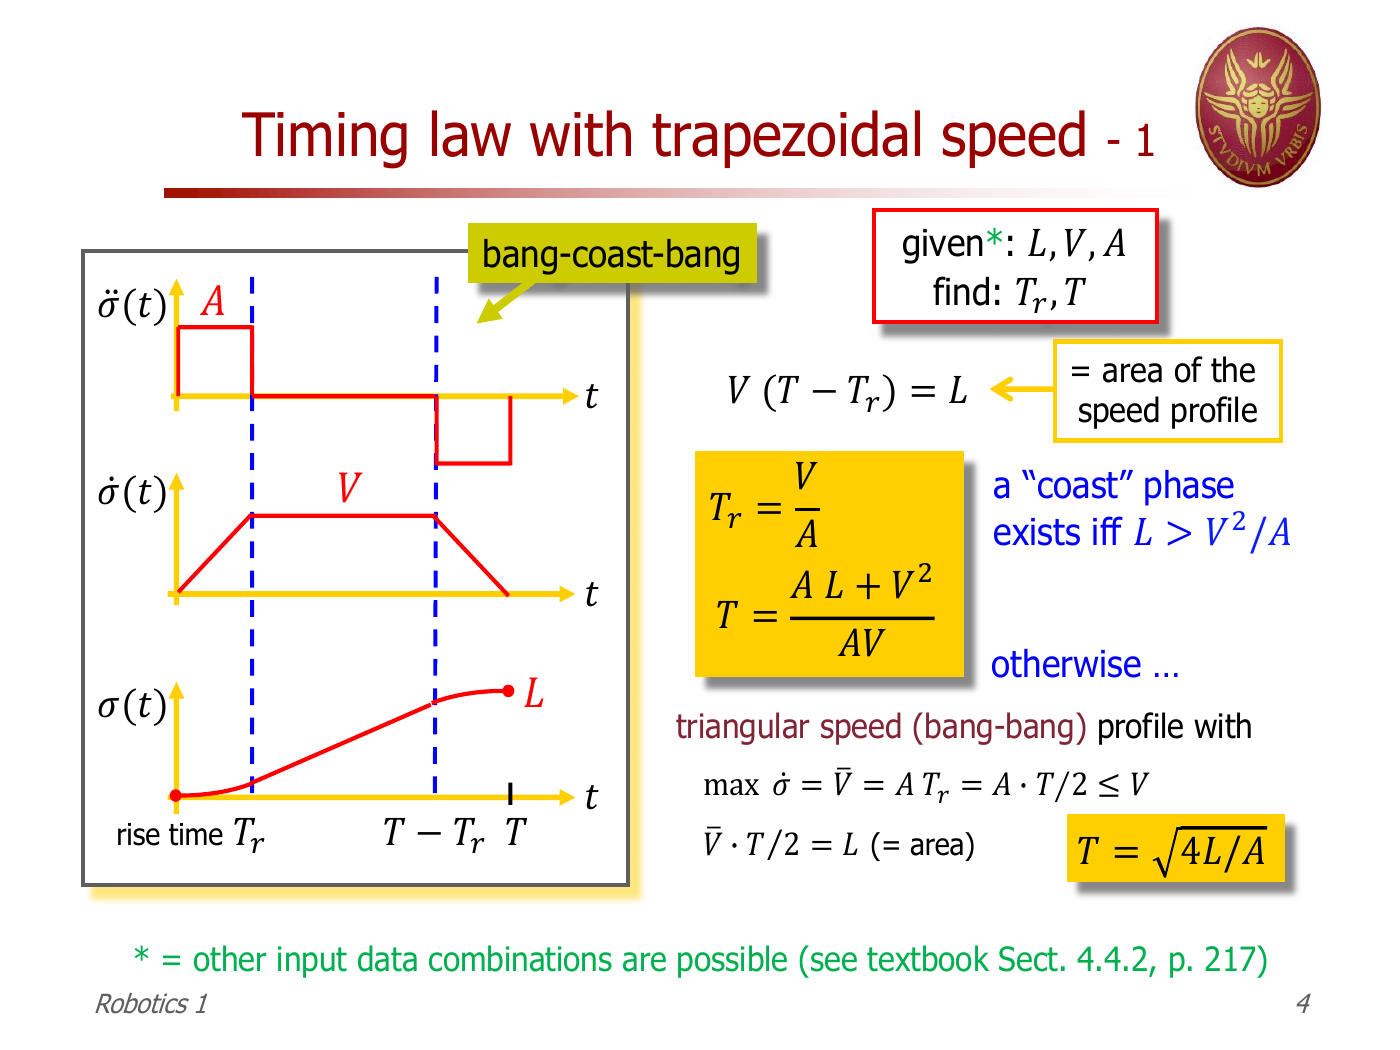
\includegraphics[width=\textwidth,height=0.8\paperheight,keepaspectratio]{dl14_p004_source.png}
\end{frame}

\begin{frame}[t]{When the trapezoid becomes a triangle}
    \small
    \begin{columns}[T,onlytextwidth]
        \begin{column}{0.49\textwidth}
            If $D<V^2/A$, the robot cannot reach $V$ before braking.
            \[V_p=\sqrt{AD}<V\]
            \[t_r=\sqrt{\frac DA},\qquad T=2\sqrt{\frac DA}\]
            In both cases:
            \[V_p=\min\bigl(V,\sqrt{AD}\bigr)\]
            At $D=V^2/A$, the plateau has zero duration.
        \end{column}
        \begin{column}{0.49\textwidth}
            \centering
            \begin{tikzpicture}[scale=0.9,>=Latex]
                \draw[->] (0,0)--(4.5,0) node[right] {$t$};
                \draw[->] (0,0)--(0,3.1) node[above] {$\dot d$};
                \draw[gray,dashed] (0,2.7)--(4.1,2.7) node[right] {$V$};
                \draw[orange,thick] (0,0)--(2,1.9)--(4,0);
                \draw[blue,thick] (0,0)--(0.6,2.7)--(1.4074,2.7)--(2.0074,0);
            \end{tikzpicture}
            \par\raggedright Same $D$ and $V$: increase $A$ to change a triangle into a trapezoid.
            \[A_{\mathrm{crit}}=\frac{V^2}{D}\]
        \end{column}
    \end{columns}
\end{frame}

\begin{frame}[t]{Live example: change the acceleration}
    \begin{figure}[H]
        \href{http://localhost:8766/W06/trajectory_demo/}{\centering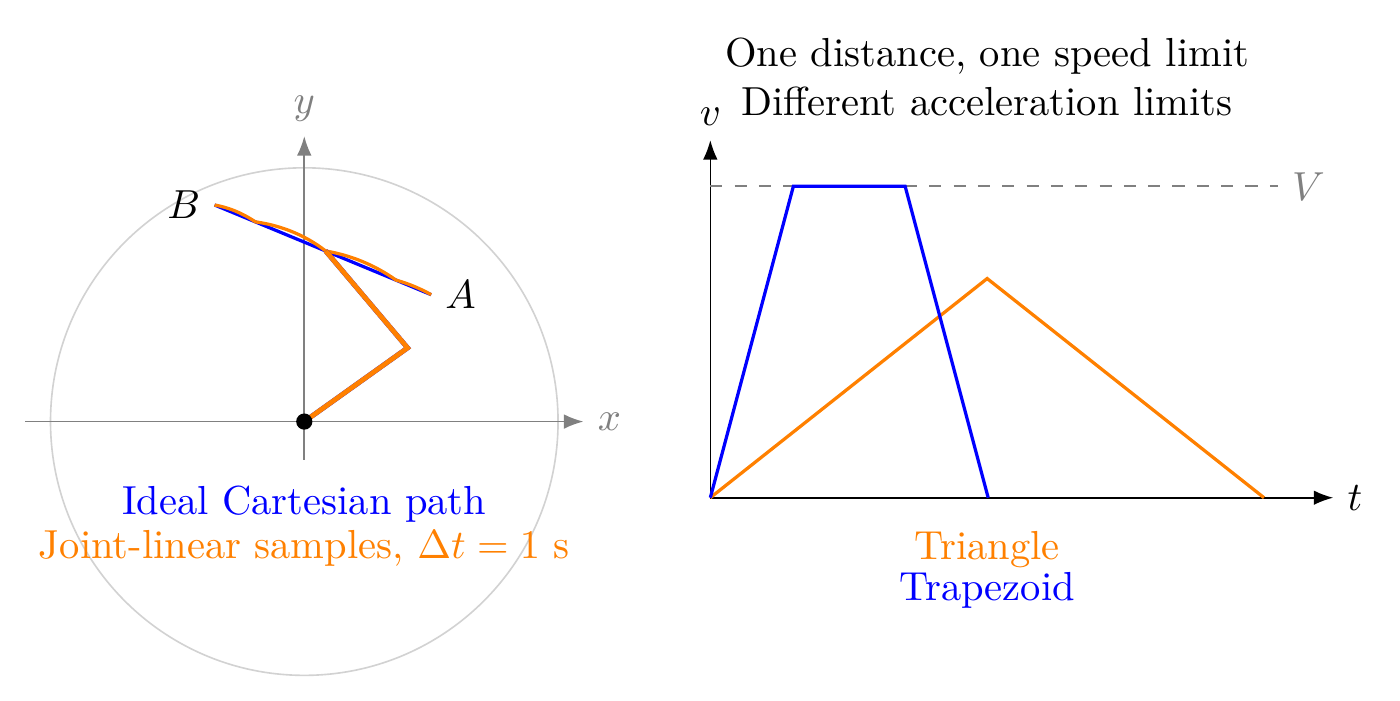
\includegraphics[height=4.4cm,width=\textwidth,keepaspectratio]{demo_preview.png}}
    \end{figure}
    \small RR: $A=(1,1)$, $B=(-\sqrt2/2,1+\sqrt2/2)$ m. Joint space: $V=60^\circ/\mathrm{s}$; compare $A=20$ and $120^\circ/\mathrm{s}^2$.
\end{frame}

\begin{frame}[t]{Problem: move an RR arm between two configurations}
    \small
    \begin{columns}[T,onlytextwidth]
        \begin{column}{0.49\textwidth}
            Two links: $l_1=l_2=1$ m.
            \[q_0=(0^\circ,90^\circ),\quad q_f=(90^\circ,45^\circ)\]
            For \textbf{each} joint:
            \[|\dot q_i|\leq60^\circ/\mathrm{s},\qquad |\ddot q_i|\leq60^\circ/\mathrm{s}^2\]
            Start and finish at rest. Follow a straight path in joint space.
            \begin{block}{Find}
                A common timing law and the total duration.
            \end{block}
        \end{column}
        \begin{column}{0.49\textwidth}
            \centering
            \begin{tikzpicture}[scale=1.25]
                \draw[blue,very thick] (0,0)--(1,0)--(1,1);
                \draw[orange,very thick] (0,0)--(0,1)--(-0.707,1.707);
                \fill (0,0) circle (2pt);
                \node[right] at (1,1) {$A$};
                \node[left] at (-0.707,1.707) {$B$};
            \end{tikzpicture}
            \par\raggedright Given FK:
            \[p=\begin{bmatrix}\cos q_1+\cos(q_1+q_2)\\ \sin q_1+\sin(q_1+q_2)\end{bmatrix}\]
        \end{column}
    \end{columns}
\end{frame}

\begin{frame}[t]{Synchronize the joints with one progress variable}
    \small
    \begin{columns}[T,onlytextwidth]
        \begin{column}{0.49\textwidth}
            \[\Delta q=(90^\circ,-45^\circ)\]
            \[q_1=90^\circ s,\qquad q_2=90^\circ-45^\circ s\]
            \[\dot q_i=\Delta q_i\dot s,\qquad \ddot q_i=\Delta q_i\ddot s\]
            \begin{block}{Preserve the joint-space line}
                The joints share the same $s(t)$ and finish together.
            \end{block}
        \end{column}
        \begin{column}{0.49\textwidth}
            \[\dot s_{\max}=\min_i\frac{\dot q_{i,\max}}{|\Delta q_i|}=\frac23\ \mathrm{s}^{-1}\]
            \[\ddot s_{\max}=\min_i\frac{\ddot q_{i,\max}}{|\Delta q_i|}=\frac23\ \mathrm{s}^{-2}\]
            Joint 1 determines both limits. Joint 2 need not reach its maximum speed.
            \medskip

            Independent fastest profiles would finish at different times.
        \end{column}
    \end{columns}
\end{frame}

\begin{frame}[t]{RR solution: a 2.5-second transfer}
    \small
    \begin{columns}[T,onlytextwidth]
        \begin{column}{0.49\textwidth}
            \[t_r=1\ \mathrm{s},\quad t_c=0.5\ \mathrm{s},\quad T=2.5\ \mathrm{s}\]
            \[s(t)=\begin{cases}
                t^2/3,&0\leq t\leq1,\\
                2t/3-1/3,&1\leq t\leq1.5,\\
                1-(2.5-t)^2/3,&1.5\leq t\leq2.5.
            \end{cases}\]
            $t$ is expressed in seconds.
            \medskip

            Peak joint velocities: $60$ and $-30^\circ/\mathrm{s}$. Acceleration magnitudes: $60$ and $30^\circ/\mathrm{s}^2$.
        \end{column}
        \begin{column}{0.49\textwidth}
            \centering
            \begin{tikzpicture}[scale=1.35]
                \draw[blue,very thick] (0,0)--(1,0)--(1,1);
                \draw[orange,very thick] (0,0)--(0,1)--(-0.707,1.707);
                \draw[teal,thick,domain=0:1,samples=50] plot ({cos(90*\x)+cos(90+45*\x)},{sin(90*\x)+sin(90+45*\x)});
                \fill (0,0) circle (2pt);
                \node[right] at (1,1) {$A$};
                \node[left] at (-0.707,1.707) {$B$};
            \end{tikzpicture}
            \par\raggedright The path is straight in joint space. The TCP path is curved: $p(t)=\mathrm{FK}(q(t))$.
        \end{column}
    \end{columns}
\end{frame}

\begin{frame}[t]{From a function to sampled commands}
    \small
    \begin{columns}[T,onlytextwidth]
        \begin{column}{0.49\textwidth}
            \[t_k=k\Delta t,\qquad q_k=q(t_k)\]
            \[\{(t_0,q_0),\ldots,(T,q_f)\}\]
            \begin{itemize}
                \item Include the endpoint exactly at $T$.
                \item A smaller step produces more commands.
                \item Specify what happens between samples.
            \end{itemize}
        \end{column}
        \begin{column}{0.49\textwidth}
            \begin{block}{Sampling is part of implementation}
                A list of configurations is not yet a complete execution method.
            \end{block}
            \ttfamily\scriptsize
            times = []\par
            k = 0\par
            while k * dt < T:\par
            \hspace*{1em}times.append(k * dt)\par
            \hspace*{1em}k += 1\par
            times.append(T)\par
            \normalfont\small
            \medskip
            The last interval may be shorter than $\Delta t$.
        \end{column}
    \end{columns}
\end{frame}

\begin{frame}[t]{Sparse samples can change the executed path}
    \begin{figure}[H]
        \href{http://localhost:8766/W06/trajectory_demo/}{\centering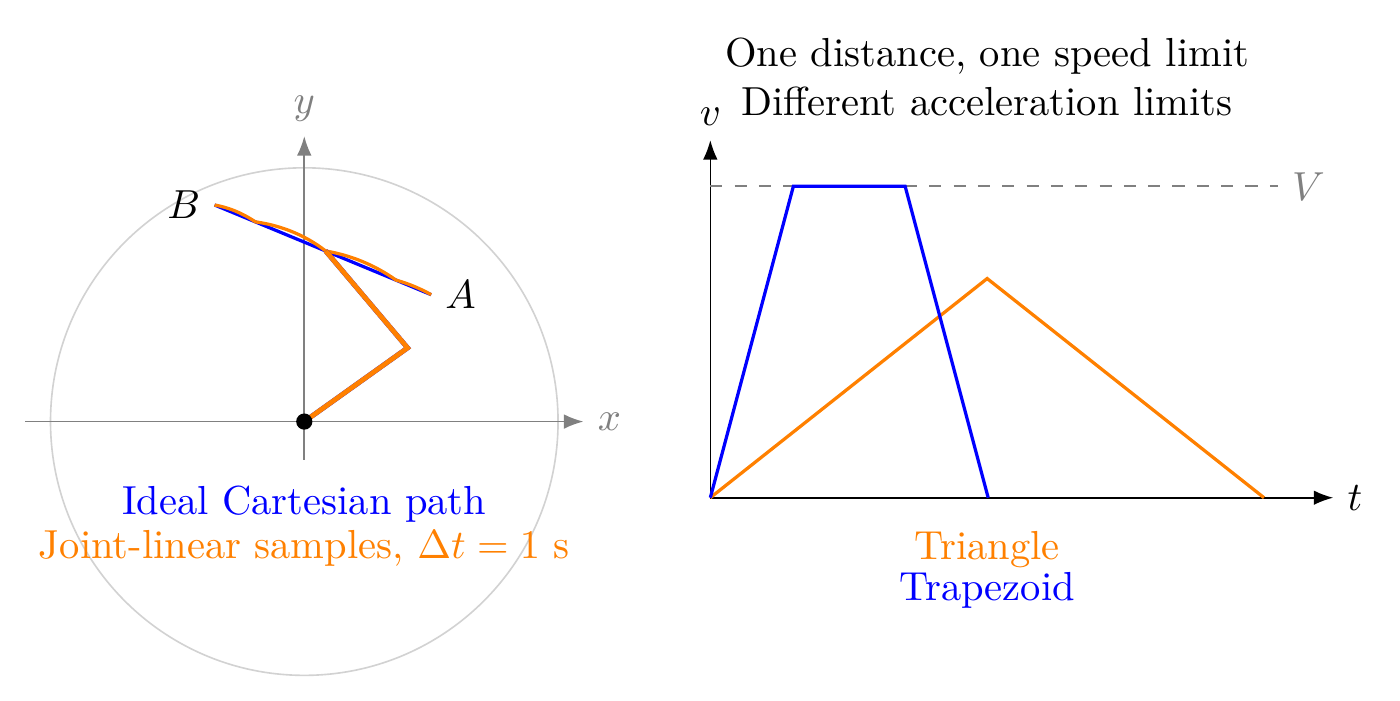
\includegraphics[height=4.1cm,width=\textwidth,keepaspectratio]{demo_preview.png}}
    \end{figure}
    \small Cartesian mode: compare $\Delta t=0.05$ and $1$ s. Blue: ideal path. Orange: joint-linear interpolation of samples. Checking samples alone can miss a collision between them.
\end{frame}

\begin{frame}[t]{Joining trajectories: stop or blend?}
    \small
    \begin{columns}[T,onlytextwidth]
        \begin{column}{0.49\textwidth}
            \textbf{Stop at the waypoint}\par
            \centering
            \begin{tikzpicture}[scale=0.6]
                \draw[blue,thick] (0,0)--(2,0)--(2,2);
                \fill (0,0) circle (2pt) node[below] {$A$};
                \fill (2,0) circle (2pt) node[below right] {$B$};
                \fill (2,2) circle (2pt) node[above] {$C$};
                \node[above] at (1,0) {$v_B=0$};
            \end{tikzpicture}
            \par
            \begin{tikzpicture}[x=0.65cm,y=0.75cm,>=Latex]
                \draw[->] (0,0)--(6.35,0) node[right] {$t$};
                \draw[->] (0,0)--(0,1.6) node[above] {$v$};
                \draw[blue,very thick] (0,0)--(1,1)--(2,1)--(3,0);
                \draw[orange,very thick] (3,0)--(4,1)--(5,1)--(6,0);
                \draw[gray,dashed] (3,0)--(3,1.45);
                \node[blue,above] at (1.5,1) {$\dot x$};
                \node[orange,above] at (4.5,1) {$\dot y$};
                \node[below] at (3,0) {$B:\ \mathbf v=0$};
            \end{tikzpicture}
            \par\raggedright\scriptsize Two consecutive trapezoids: brake to zero, then accelerate again.
        \end{column}
        \begin{column}{0.49\textwidth}
            \textbf{Blend around the waypoint}\par
            \centering
            \begin{tikzpicture}[scale=0.6]
                \draw[gray,dashed] (0,0)--(2,0)--(2,2);
                \draw[orange,thick] (0,0)--(1.5,0);
                \draw[orange,thick,domain=0:1,samples=25] plot ({1.5+\x-0.5*\x*\x},{0.5*\x*\x});
                \draw[orange,thick] (2,0.5)--(2,2);
                \fill (0,0) circle (2pt) node[below] {$A$};
                \fill (2,0) circle (2pt) node[below right] {$B$};
                \fill (2,2) circle (2pt) node[above] {$C$};
            \end{tikzpicture}
            \par
            \begin{tikzpicture}[x=0.65cm,y=0.75cm,>=Latex]
                \fill[green!12] (2,0) rectangle (3,1.45);
                \draw[->] (0,0)--(6.35,0) node[right] {$t$};
                \draw[->] (0,0)--(0,1.6) node[above] {$v$};
                \draw[blue,thick,dashed] (0,0)--(1,1)--(2,1)--(3,0);
                \draw[orange,thick,dashed] (2,0)--(3,1)--(4,1)--(5,0);
                \draw[green!45!black,very thick] (0,0)--(1,1)--(2,1);
                \draw[green!45!black,very thick,domain=2:3,samples=41] plot (\x,{sqrt((3-\x)^2+(\x-2)^2)});
                \draw[green!45!black,very thick] (3,1)--(4,1)--(5,0);
                \draw[gray,dashed] (2,0)--(2,1.45) (3,0)--(3,1.45);
                \node[blue,above] at (1.5,1) {$\dot x$};
                \node[orange,above] at (3.5,1) {$\dot y$};
                \node[below] at (2.5,0) {$\Delta T$};
                \node[green!45!black,right] at (4.25,1.3) {$\|\mathbf v\|$};
            \end{tikzpicture}
            \par\raggedright\scriptsize The resultant speed rolls between the two profiles: $\min\|\mathbf v\|=V/\sqrt2>0$.
        \end{column}
    \end{columns}
    \smallskip
    \scriptsize Blue: $\dot x$; orange: $\dot y$. Green: resultant speed through the blend. Perpendicular segments.\\
    \alert{Blending changes the path: check clearance again.}
\end{frame}

\begin{frame}[c]
    \centering
    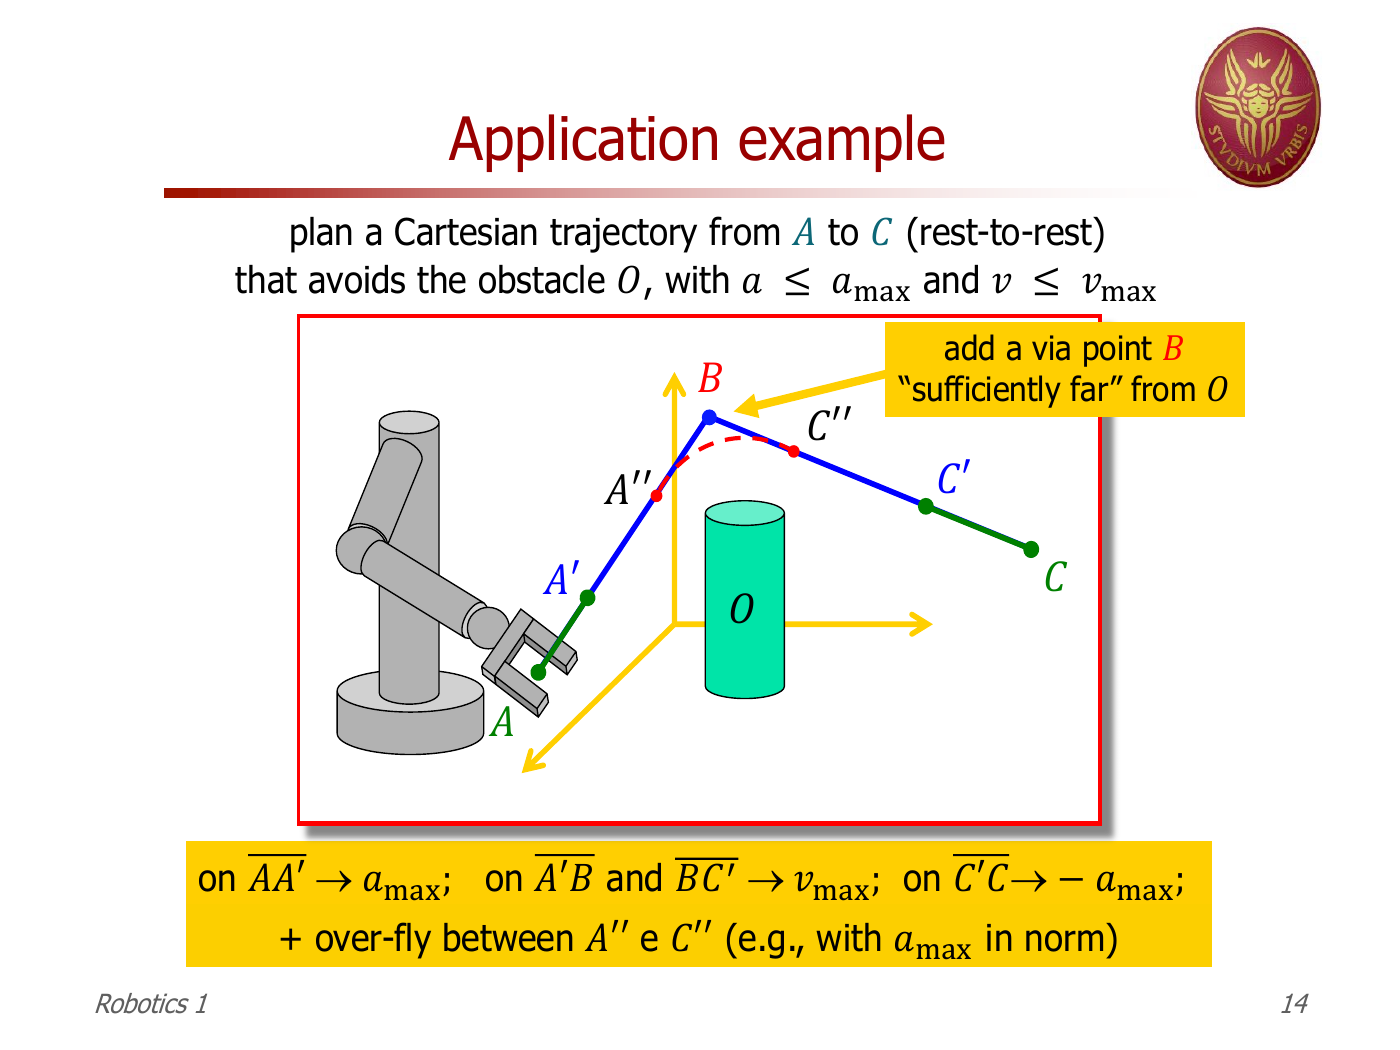
\includegraphics[width=\textwidth,height=0.8\paperheight,keepaspectratio]{dl14_p014_source.png}
\end{frame}

\begin{frame}[t]{What we will observe on the UR5}
    \begin{columns}[T,onlytextwidth]
        \begin{column}{0.49\textwidth}
            \begin{enumerate}
                \item Joint jogging and TCP movement.
                \item Base and tool coordinate frames.
                \item Freedrive and stored waypoints.
            \end{enumerate}
        \end{column}
        \begin{column}{0.49\textwidth}
            \begin{enumerate}\setcounter{enumi}{3}
                \item MoveJ versus MoveL.
                \item Speed, acceleration and duration.
                \item Stopping versus blending.
            \end{enumerate}
        \end{column}
    \end{columns}
    \medskip
    Same targets $\to$ different paths.\\
    Same path $\to$ different motion times.
\end{frame}

\begin{frame}[t]{Reference Materials}
    \begin{itemize}
        \item A. De Luca --- 13 TrajectoryPlanning
        \item A. De Luca --- 06 ProgrammingArchitectures
        \item O. Bulichev --- Tactile sensing experiments with a UR manipulator
        \item A. Klimchik --- L13 Trajectory planning
        \item A. De Luca --- 14 TrajectoryPlanningCartesian
        \item Universal Robots --- Programming and communication interfaces
        \item Universal Robots --- Motion primitives
        \item Universal Robots --- Teaching and manual movement
        \item Kavraki Lab --- Sampling-based motion planning in OMPL
        \item NVIDIA --- cuRobo motion generation
    \end{itemize}
\end{frame}


\fbckg{fibeamer/figs/last_page.png}
\frame[plain]{}

\end{document}
